
\documentclass{article} % For LaTeX2e
\usepackage{iclr2026_conference,times}

% Optional math commands from https://github.com/goodfeli/dlbook_notation.
\input{math_commands.tex}

\usepackage{hyperref}
\usepackage{url}
\usepackage[utf8]{inputenc} % allow utf-8 input
\usepackage[T1]{fontenc}% use 8-bit T1 fonts
\usepackage{hyperref}% hyperlinks
\usepackage{url} % simple URL typesetting
\usepackage{booktabs}% professional-quality tables
\usepackage{amsfonts}% blackboard math symbols
\usepackage{subfig}  % for \subfloat
\usepackage[table]{xcolor} % for \cellcolor
\usepackage{nicefrac}% compact symbols for 1/2, etc.
\usepackage{microtype}  % microtypography
\usepackage{xcolor}  % colors
\usepackage{amsmath}
\usepackage{multirow}
\usepackage{graphicx}
\usepackage{caption}
\usepackage{wrapfig}
\usepackage{tabularx}
\usepackage[normalem]{ulem}
\useunder{\uline}{\ul}{}
\usepackage[margin=1in]{geometry}
\usepackage{amsmath,amssymb,amsfonts}
\usepackage{bm}
\usepackage{algorithm}
\usepackage{algpseudocode}
\usepackage{xcolor}
\usepackage{xspace}
\usepackage{booktabs}
\usepackage{graphicx}




% ---- light formatting helpers ----
\algrenewcommand\algorithmicrequire{\textbf{Input:}}
\algrenewcommand\algorithmicensure{\textbf{Output:}}
\newcommand{\COMMENT}[1]{\hfill\textcolor{gray}{$\triangleright$ \footnotesize #1}}
\algnewcommand{\LineComment}[1]{\State \textcolor{gray}{$\triangleright$ \footnotesize #1}}
 
% ---- math shortcuts ----
\newcommand{\method}{\textsc{HarnessRL}\xspace}
\newcommand{\sftm}{\operatorname{softmax}}
\newcommand{\score}{\operatorname{score}}
\newcommand{\TopK}{\operatorname{Top\text{-}\kappa}}
\newcommand{\Dtok}{\mathcal{D}_{\mathrm{tok}}}
\newcommand{\Dord}{\mathcal{D}_{\mathrm{ord}}}
\newcommand{\Smask}{\mathcal{S}_t}
\newcommand{\Cand}{\mathcal{C}_t}

 
% \usepackage[numbers,square]{natbib} %
\newcommand{\chaowei}[1]{\textcolor{cyan}{[Chaowei: #1]}}

\title{Learning the Harness, Not the Weights: \\
Reinforcement Learning of a Harness Proposer \\
for Frozen-Executor Discovery Agents}

% Authors must not appear in the submitted version. They should be hidden
% as long as the \iclrfinalcopy macro remains commented out below.
% Non-anonymous submissions will be rejected without review.

\author{Antiquus S.~Hippocampus, Natalia Cerebro \& Amelie P. Amygdale \thanks{ Use footnote for providing further information
about author (webpage, alternative address)---\emph{not} for acknowledging
funding agencies.  Funding acknowledgements go at the end of the paper.} \\
Department of Computer Science\\
Cranberry-Lemon University\\
Pittsburgh, PA 15213, USA \\
\texttt{\{hippo,brain,jen\}@cs.cranberry-lemon.edu} \\
\And
Ji Q. Ren \& Yevgeny LeNet \\
Department of Computational Neuroscience \\
University of the Witwatersrand \\
Joburg, South Africa \\
\texttt{\{robot,net\}@wits.ac.za} \\
\AND
Coauthor \\
Affiliation \\
Address \\
\texttt{email}
}

% The \author macro works with any number of authors. There are two commands
% used to separate the names and addresses of multiple authors: \And and \AND.
%
% Using \And between authors leaves it to \LaTeX{} to determine where to break
% the lines. Using \AND forces a linebreak at that point. So, if \LaTeX{}
% puts 3 of 4 authors names on the first line, and the last on the second
% line, try using \AND instead of \And before the third author name.

\newcommand{\fix}{\marginpar{FIX}}
\newcommand{\new}{\marginpar{NEW}}

%\iclrfinalcopy % Uncomment for camera-ready version, but NOT for submission.
\begin{document}


\maketitle

\begin{abstract}
The behavior of an LLM agent is a property of the coupled model--harness
system: the prompts, skills, tools, and control loop around the weights
decide how much of the model's capability becomes measurable progress.  On
discovery tasks---where an agent iteratively edits a program against a
black-box evaluator---strong harnesses are today hand-engineered per domain,
and the alternative, finetuning the model for discovery, is unavailable
whenever the executor is frozen by policy or served behind an API.  We argue
that harness design is itself a learnable skill.  We introduce \method{},
which trains a harness \emph{proposer}---the executor's own base model with a
LoRA adapter---by group-relative reinforcement learning to synthesize
complete, task-conditioned harnesses: system prompts, skill playbooks, tool
descriptions, control parameters, and, through a generative channel,
\emph{new executable tools} written as Python.  Each proposed spec compiles
into a runnable agent package, is rolled out by the permanently frozen
executor under a hard evaluator budget, and the group's relative outcomes are
the only training signal.  Because the optimizer may now write code that runs
inside the evaluation loop, generated tools pass a leakage-controlled review
chain: a capability-bounded SDK that cannot reach the evaluator, fail-closed
static gates, and a repairer with \emph{capability parity}---the same frozen
model, localization-guarded---that can fix code but not smuggle knowledge.
Discovery also breaks the standard GRPO recipe, so we derive a group
objective with gap-normalized rewards, a leave-one-out baseline, and
max-weighted sharpening aligned with best-of-$K$ selection.  With 27 RL
steps under a pre-registered 30-step cap, the learned proposer carries a
frozen 9B executor past a discovery-finetuned model of the same scale on
\textbf{all eleven} tasks of a suite spanning mathematical construction,
systems algorithm design, and heuristic-contest programming---by up to
$15\%$---and past the published $\le$10B state of the art on PRISM (25.59
vs.\ 24.70), while the same executor under a fixed hand-written harness
clears only 3 of 11.  A breakthrough ledger traces every jump in the
campaign to an identifiable mechanism---sampling breadth, compounding
inheritance, or new information reaching the system---separating what the RL
learned from what the search found.
\end{abstract}


\section{Introduction}
\label{sec:introduction}

Large language models act in the world through \emph{agents}: a model embedded
in a harness---the software that supplies its system prompt, tools, skills,
context policy, and control loop~\citep{weng2026harness,anthropicagents,react,
toolformer,sweagent,autogen,voyager,webarena,osworld}.  How much of a model's
capability becomes measurable progress is decided by that harness, nowhere more
sharply than in \emph{discovery}, where a frozen LLM paired with a hand-built
evolutionary scaffold produces mathematical and algorithmic results beyond
strong baselines~\citep{funsearch,alphaevolve,alphaevolvemath,openevolve,
shinkaevolve,eoh,llmsr,aiscientist}.  A natural next step is
\emph{self-improvement}: letting an agent get better at a task from its own
experience, with no stronger model to learn from.  Today this takes one of two
forms (Figure~\ref{fig:taxonomy}a,b).  One updates the model's \emph{weights},
fine-tuning the executor on its own rollouts, as in test-time and reasoning
RL~\citep{tttdiscover,thetaevolve,ttrl,ttt,grpo,dapo,agenticrl,ragen}.  The
other keeps the model frozen and edits its \emph{harness}---prompts, tools,
context, or an external program archive---as an artifact revised by a
\emph{fixed} proposer~\citep{openevolve,funsearch,shinkaevolve,eoh,metaharness,
selfharness,hase,dgm,sica,godelagent,stop,alita,selfevolvesurvey}.

\begin{figure*}[t]
\centering
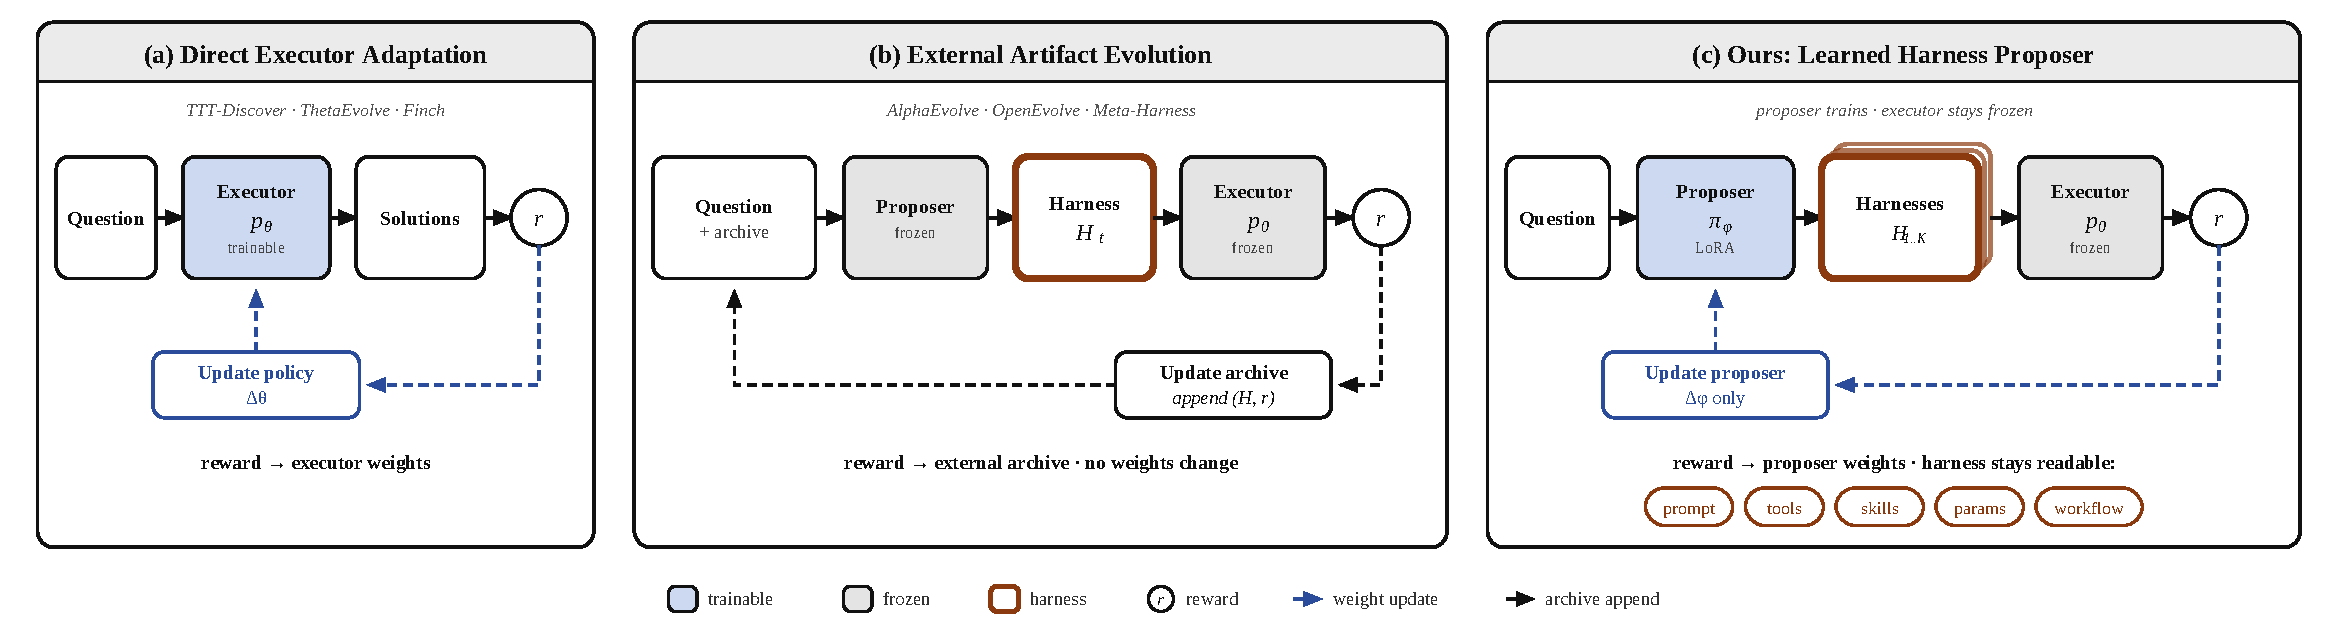
\includegraphics[width=\textwidth]{figures/harness_taxonomy.pdf}
\caption{\textbf{Where does the reward go?}  Three ways to improve an agent from
its own experience.  \textbf{(a)}~\emph{Direct executor adaptation}
(TTT-Discover, ThetaEvolve, Finch): the reward updates the executor's own
weights, so the policy that solves the task is also the policy that is trained.
\textbf{(b)}~\emph{External artifact evolution} (AlphaEvolve, OpenEvolve,
Meta-Harness): the executor stays frozen and the reward is appended to an
external archive or harness, which a \emph{fixed} proposer reads back.
\textbf{(c)}~\emph{\method{} (ours)}: a trainable proposer emits harnesses
$H_{1:K}$---prompt, tool descriptions, skills, and control parameters---for a permanently
frozen executor, and only the proposer is updated.  Adaptation is thus separated
from execution and routed through an explicit, inspectable artifact.}
\label{fig:taxonomy}
\end{figure*}

Both routes stop short of a reusable \emph{proposer}, in complementary ways.
Weight updates train on hundreds of rollouts per
step~\citep{tttdiscover,thetaevolve}, register their gains only as diffuse
weight changes---never as a nameable tool, skill, or procedure---and are
unavailable when the executor is frozen by policy, safety review, or an API
boundary.  Harness editing keeps its \emph{proposer} fixed: the same
prompt-optimizer, textual-gradient, or agent-design
procedure~\citep{ape,opro,promptbreeder,evoprompt,mipro,metaprompting,dspy,
textgrad,trace,gepa,adas,aflow,agentsquare,agentsymbolic} re-derives design
knowledge from scratch on every run, with nothing amortized into the
proposer itself.  History suggests the resolution: hand-designed pipelines
gave way to searched ones, and searched ones to \emph{learned}
components~\citep{learn2learn,hypernetworks,adas}.

We propose to learn the proposer itself (Figure~\ref{fig:taxonomy}c).
\method{} keeps the executor $M_0$ \textbf{permanently frozen} and trains a
harness \emph{proposer} $\pi_\phi$ by group-relative RL adapted for
discovery (\S\ref{sec:method}) to emit, per task, a complete harness:
system prompt, skill playbook, tool descriptions, control parameters, and,
through a generative channel, \emph{new executable tools} as Python
source~\citep{latm,creator,craft,voyager,trove}.  Each spec compiles
deterministically into a runnable agent; the frozen executor rolls it out
under a hard evaluator budget; and a group's relative outcomes are the
proposer's only task-level signal (Figure~\ref{fig:overview}).  Round over
round, the proposer internalizes the task's reward history into its weights
rather than into an ever-growing context.

Three properties motivate this design.  \emph{Amortization}: search cost
is paid at training time, so a new round costs a handful of proposer
episodes rather than a fresh scaffold search---the argument behind learned
optimizers and hypernetworks~\citep{learn2learn,hypernetworks}.
\emph{Expressiveness}: the generative channel carries executable code, so a
proposed agent can differ from its siblings in what machinery exists, not
only in how it is described~\citep{adas,latm,voyager}.  \emph{Attribution
and safety}: freezing $M_0$ makes each improvement attributable to an
inspectable harness---but machine-written code inside an evaluation loop
invites reward hacking~\citep{skalse2022,specgaming,denison2024,baker2025,
metr2025,impossiblebench}, so generated tools cannot read the evaluator or
ground truth, pass fail-closed gates and sandboxed self-tests, and are
repaired only by \emph{the same frozen model} under a localization guard
(\S\ref{sec:method-safety}).

We evaluate on eleven hard problems---AlphaEvolve-style mathematical
constructions~\citep{alphaevolve,alphaevolvemath}, four systems benchmarks
from the ADRS suite~\citep{barbarians}, and two AtCoder Heuristic Contest
problems~\citep{ahc,alebench}---the suite whose discovery-finetuned Finch
models we take as the matched-scale baseline~\citep{finch}.  Under a budget
of at most 30 RL steps fixed in advance, the learned proposer's harnesses
carry a frozen 9B executor~\citep{qwen3} past Finch-9B on \textbf{all
eleven} tasks and set the published $\le$10B state of the art on
\textbf{five}: Erd\H{o}s minimum overlap, ahc039, ahc058, EPLB, and PRISM
(a sixth, LLM-SQL, exceeds the prior best but traces to a curated note and
is excluded from every claim, \S\ref{sec:exp-results}); the same executor
under the fixed initial harness beats Finch-9B on only two
(Table~\ref{tab:conditions}).  The Erd\H{o}s record---previously held by
test-time RL that adapts the executor
directly~\citep{tttdiscover,thetaevolve}---now falls to a frozen executor,
which also surpasses the best known human construction ($0.380919$ vs.\
$0.380927$) with a step-function optimizer it wrote itself, under a harness
that named no such method.  Much of what reads as a small model's
capability ceiling is a harness that has not told the executor what game it
is playing; the remedy is a change of harness, not a larger model.

\section{Problem Statement}
\label{sec:problem}

\begin{figure}[t]
\centering
% TODO(figure): replace placeholder. Intended content — left: proposer
% pi_phi (frozen base + LoRA) reads task context c_tau (task spec, incumbent
% program/harness, experience digest) and emits K harness specs; middle:
% review chain for generated tools (static gates -> sandboxed self-test ->
% capability-parity repair) feeding the materializer, which compiles K agent
% packages (prompt, skills, tool schemas, custom tool code); right: frozen
% M_0 rolls each package out from the inherited program under budget B;
% scores -> gap-normalized group advantages -> GRPO update of phi; incumbents
% ratchet and feed the next round's context.
\framebox[\textwidth]{\parbox{0.94\textwidth}{\centering\vspace{16mm}
\textit{Figure placeholder: \method{} overview --- proposer episodes
$\to$ tool review chain $\to$ materialized agent packages $\to$ frozen-executor
rollouts $\to$ group-relative update; incumbents ratchet across rounds.}
\vspace{16mm}}}
\caption{\textbf{Overview of \method{}.}  A LoRA proposer $\pi_\phi$,
conditioned on the task and on digested experience from previous rounds,
emits $K$ harness specs per task.  Generated tools pass a leakage-controlled
review chain before the spec is compiled into a runnable agent package.  The
permanently frozen executor $M_0$ rolls out each package from the incumbent
best program under a hard evaluator budget; group-relative advantages update
$\phi$, and per-task incumbents (best program, best harness) ratchet forward
to condition the next round.}
\label{fig:overview}
\end{figure}

\paragraph{Agents and harnesses.}  An agent is a pair $\Phi = (M, H)$ of a
language model $M$ and a harness $H$.  In our setting the harness is a
concrete, typed object
$H = (P,\, S,\, D,\, \theta,\, T)$: a system prompt $P$; a skill package $S$
loaded into context; descriptions $D$ of the agent's tools (the behavioral
interface through which $M$ understands its own machinery); control
parameters $\theta$ (sampling temperature, top-$p$, iteration caps,
middleware thresholds); and a tool set $T = T_{\mathrm{fixed}} \cup
T_{\mathrm{gen}}$, where $T_{\mathrm{fixed}}$ are built-in executor tools and
$T_{\mathrm{gen}}$ are \emph{generated} tools shipped as Python source and
compiled into the agent.  Prior scaffold-optimization work searches subsets
of this object---prompts~\citep{opro,gepa}, workflow
graphs~\citep{aflow,agentsquare}, or agent code~\citep{adas,dgm}; we treat
the full tuple as the output of a learned policy.

\paragraph{Discovery tasks.}  A task $\tau = (d_\tau, x_0, \mu_\tau, B)$
consists of a natural-language description $d_\tau$, a seed program $x_0$
with an editable region, a black-box evaluator $\mu_\tau$ returning a scalar
score, and a hard budget of $B$ evaluator calls.  Running agent
$(M_0, H)$ on $\tau$ produces an edit$\to$evaluate trajectory; its outcome
is the best score reached within budget,
$s(\tau, H) = \max_{t \le B}\, \mu_\tau(x_t)$.
This regime---iterative program improvement against an oracle
score---underlies FunSearch, AlphaEvolve, and their
successors~\citep{funsearch,alphaevolve,shinkaevolve}, where the loop around
the model, not the model, is the designed object.

\paragraph{Learned harness synthesis.}  The executor $M_0$ is frozen: its
weights never change, whether by finetuning or test-time
training~\citep{ttt,ttrl}.  Improvement is delegated to a \emph{proposer}
policy $\pi_\phi(z \mid c_\tau)$ that emits a harness spec $z$ (compiled to
$H_z$ by a deterministic materializer) conditioned on a task context
$c_\tau$ containing $d_\tau$, the incumbent best program and harness, and
digested telemetry from earlier rounds.  The learning problem is
\begin{equation}
\max_\phi \;\; \mathbb{E}_{\tau \sim \mathcal{T}} \;
\mathbb{E}_{z \sim \pi_\phi(\cdot \mid c_\tau)}
\big[\, s(\tau, H_z) \,\big],
\label{eq:objective}
\end{equation}
optimized with group-relative RL over $K$ proposer episodes per task per
round.  Two properties distinguish
Eq.~\eqref{eq:objective} from per-task scaffold search~\citep{adas,gepa,
aflow}: the trained object is the \emph{proposer}, so design knowledge
amortizes across tasks and rounds; and because $z$ includes executable
code, the reachable harness family is not enumerable in advance.  Two
properties distinguish it from executor RL~\citep{grpo,agenticrl}: no
gradient touches $M_0$, and the reward is an \emph{outer} quantity---the
best score of an entire inner agent trajectory, not a per-token or
per-answer signal.

\emph{The core difficulty is credit assignment through two nested loops: a
scalar that summarizes an entire frozen-executor rollout must teach the
proposer which of its design decisions---a prompt clause, a control
parameter, a generated tool---mattered, under evaluator noise and a rollout
budget too small to average it away.}  \method{}'s answer combines a typed
spec space that makes decisions legible (\S\ref{sec:method-genome}), a
review chain that keeps generated code from corrupting the measurement
(\S\ref{sec:method-safety}), and a group objective shaped for best-of-$K$
discovery rather than mean-seeking preference tuning
(\S\ref{sec:method-rl}).

\section{\method{}}
\label{sec:method}

\begin{figure*}[t]
\centering
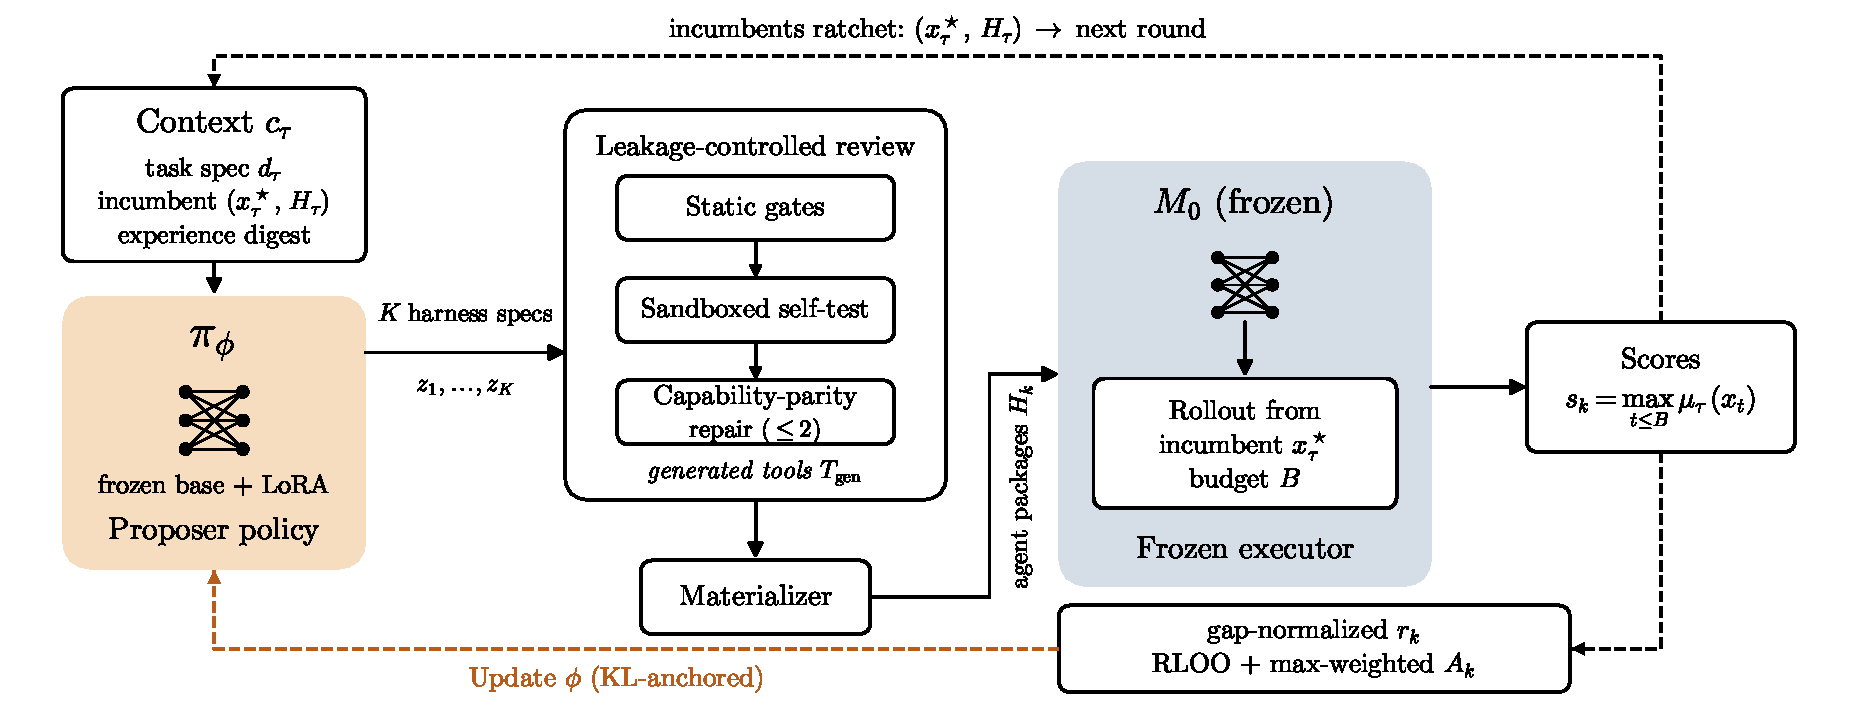
\includegraphics[width=\textwidth]{figures/overview_1.pdf}
\caption{\textbf{Overview of \method{}.}  \emph{Outer loop:} a proposer
$\pi_\phi$---the executor's own frozen base plus a LoRA adapter, the only
trained component---reads a task context $c_\tau$ (task spec, incumbent program
and harness, and a digest of what every previous candidate did, scored, and died
of) and emits $K$ harness specs.  Generated tool code passes a leakage-controlled
review chain (fail-closed static gates, sandboxed self-test, and repair held to
capability parity with the executor) before a deterministic materializer compiles
each spec into a runnable agent package $H_k$.  \emph{Inner loop:} the
permanently frozen executor $M_0$ rolls out each package from the incumbent
program under a hard evaluator budget $B$.  Two feedback paths close the loop:
the group's scores become gap-normalized rewards and RLOO advantages that update
\emph{only} $\phi$, and the round's best program and harness ratchet forward into
the next round's context.  Nothing in this loop updates $M_0$.}
\label{fig:overview}
\end{figure*}

\subsection{Setup and objective}
\label{sec:method-setup}

An agent is a pair $\Phi = (M, H)$ of a language model $M$ and a harness $H$.
We treat the harness as a concrete, typed object
$H = (P,\, S,\, D,\, \theta,\, T)$: a system prompt $P$; a skill package $S$
loaded into context; descriptions $D$ of the agent's tools (the behavioral
interface through which $M$ understands its own machinery); control parameters
$\theta$ (sampling temperature, iteration caps, middleware thresholds); and a
tool set $T = T_{\mathrm{fixed}} \cup T_{\mathrm{gen}}$, where
$T_{\mathrm{gen}}$ are \emph{generated} tools shipped as Python source and
compiled into the agent.  Prior scaffold optimization searches subsets of this
object---prompts~\citep{opro,gepa}, workflow graphs~\citep{aflow,agentsquare},
or agent code~\citep{adas,dgm}; we treat the full tuple as the output of a
learned policy.

A task $\tau = (d_\tau, x_0, \mu_\tau, B)$ consists of a natural-language
description, a seed program with an editable region, a black-box evaluator
returning a scalar score, and a hard budget of $B$ evaluator calls.  Running
$(M_0, H)$ on $\tau$ produces an edit$\to$evaluate trajectory whose outcome is
the best score reached within budget,
$s(\tau, H) = \max_{t \le B}\, \mu_\tau(x_t)$, where $x_t$ is the program
after $t$ edits from the round's start program.  Rounds inherit the incumbent rather than the seed
(\S\ref{sec:method-search}), so a valid candidate's score is floored at the
incumbent's and the reward below is non-negative except for invalid candidates.  The executor $M_0$ is frozen:
its weights never change, whether by fine-tuning or by test-time
training~\citep{ttt,ttrl}.  Improvement is delegated to a proposer
$\pi_\phi(z \mid c_\tau)$ that emits a harness spec $z$---compiled to $H_z$ by a
deterministic materializer---conditioned on a context $c_\tau$ holding
$d_\tau$, the incumbent best program and harness, and digested telemetry from
earlier rounds.  The learning problem is
\begin{equation}
\max_\phi \;\; \mathbb{E}_{\tau \sim \mathcal{T}} \;
\mathbb{E}_{z \sim \pi_\phi(\cdot \mid c_\tau)}
\big[\, s(\tau, H_z) \,\big],
\label{eq:objective}
\end{equation}
optimized with group-relative RL over $K$ proposer episodes per task per round.
What separates this formulation from per-task scaffold
search~\citep{adas,gepa,aflow,dgm} is the trained object: the \emph{proposer}
itself, so design knowledge amortizes across tasks and rounds instead of being
re-derived per task.  Like ADAS and the Darwin G\"odel Machine, and unlike
prompt- or graph-level search~\citep{gepa,aflow}, our search space carries
executable code, so the reachable harness family is not enumerable in advance.
Two more separate it from executor RL~\citep{grpo,agenticrl}: no gradient
touches $M_0$, and the reward is an \emph{outer} quantity---the best score of an
entire inner trajectory, not a per-token signal.

\emph{The core difficulty is credit assignment through two nested loops: a
scalar summarizing an entire frozen-executor rollout must teach the proposer
which of its design decisions---a prompt clause, a control parameter, a
generated tool---mattered, under evaluator noise and a rollout budget too small
to average it away.}  The rest of this section follows one round through the
system (Algorithm~\ref{alg:outer}): a typed spec space that makes decisions
legible (\S\ref{sec:method-genome}), a review chain that keeps generated code
from corrupting the measurement (\S\ref{sec:method-safety}), and a group
objective shaped for best-of-$K$ discovery (\S\ref{sec:method-rl}).

\subsection{The harness genome}
\label{sec:method-genome}
Candidates are expressed in a typed, fail-closed spec language rather than
free-form code: every submission either validates---and compiles into a
runnable package---or is rejected with a machine-readable error that flows
back into the proposer's next context.  \emph{Declarative} fields
reconfigure fixed machinery: the executor's system prompt, the skill
playbook, the descriptions of the fixed tools, sampling parameters, the
iteration cap, and middleware thresholds (budget reminders, stall-triggered
restarts, output truncation).  \emph{Generative} fields extend the machinery
itself: up to three \texttt{new\_tools}---each a name, description, JSON
input schema, and Python implementation---plus up to two new skills, up to two
\texttt{new\_middlewares} (a hook and a Python implementation each), and the
removal of designated optional tools.  Unlike tool-\emph{use}
pipelines~\citep{toolformer,toolllm} and library-induction methods that
abstract tools from solution traces~\citep{latm,creator,craft,trove,
voyager}, tools here are authored by the \emph{proposer} policy as part of a
harness, before the executor ever runs, and become first-class members of
the compiled agent.  A deterministic materializer turns a validated spec
into a complete package---prompt, skill files, tool schemas,
\texttt{custom\_tools/*.py} bound to a runtime dispatcher---so identical
specs yield byte-identical agents (modulo provenance metadata) and a spec hash de-duplicates candidates
within a group.

\paragraph{An experience-conditioned proposer.}
The proposer is itself a small agent: $\pi_\phi$ (frozen base plus LoRA)
runs inside a fixed two-tool harness (\texttt{validate\_spec},
\texttt{submit\_spec}) for one episode per candidate.  Its context $c_\tau$
carries the task description, an excerpt of the incumbent best program, the
incumbent spec and score, and an \emph{experience digest}: for every
candidate of the previous visit, its score, evaluator calls, stop reason,
changed fields, validation errors, and per-tool review outcomes, plus an
optional curated analyst note about the scoring rule
(\S\ref{sec:method-search}).  The $K$ episodes for a task share $c_\tau$ and
differ only in sampling seed, forming a single group for the group-relative update.  Feeding outcomes back
as language---rather than only as scalars---echoes reflective
optimization~\citep{reflexion,gepa,trace}; the difference is that here the
reflection loop trains a persistent policy, so design knowledge accumulates
in weights rather than in a per-task search state.

\subsection{Leakage-controlled tool generation}
\label{sec:method-safety}

Letting the proposer write code that runs inside the evaluation loop
invites the classic failure modes of specification
gaming~\citep{skalse2022,specgaming}: a tool that reads the evaluator or
answer files hacks the reward outright~\citep{denison2024,baker2025,
impossiblebench}, and a repair pathway routed through a strong model can
\emph{leak} solution knowledge into the executor's context, corrupting the
claim that the frozen executor did the discovering.  \method{} closes both
channels by construction, in four layers.
\textbf{(1) Capability surface:} a generated tool implements a single
\texttt{run(ctx, args)} entry point and touches the world only through
\texttt{ctx}---staged edits, cheap subsampled probes, budgeted evaluation,
task-input samples, scratch space.  The evaluator's implementation, the ground
truth, and the network are unreachable through this surface, and the static gates
below enforce the same boundary independently (the full capability surface is
listed in Appendix~\ref{app:sdk}).
\textbf{(2) Static gates:} a fail-closed AST pass enforces an import
whitelist, forbids \texttt{os}/\texttt{subprocess}/\texttt{open}/%
\texttt{exec}/dunder access, and requires the exact entry signature;
survivors execute against a mock context in an rlimit-sandboxed subprocess.
\textbf{(3) Capability-parity repair:} tools that fail enter a bounded
repair loop ($\le 2$ rounds) whose repairer is \emph{the same frozen served
model} as the executor---never a stronger external model---so the reviewer
cannot inject knowledge the executor lacks.  The repair prompt carries only
the code and the error (a scrubber rejects prompts containing evaluator or
target-score content), and a \emph{localization guard} rejects repairs whose
similarity to the original falls below $0.55$: a rewrite is treated as
attempted knowledge injection, not a fix.
\textbf{(4) Fail-closed accounting:} repaired code is re-gated and
re-tested; tools that never pass are dropped, and a candidate left without
any effective mutation is invalidated.  The review outcome of every tool is
reported back to the proposer in the next experience digest.

\subsection{A group objective for discovery}
\label{sec:method-rl}

Group-relative policy optimization was built for preference and
reasoning tuning, where rewards share a scale and the mean group outcome is
the target~\citep{grpo,rloo}.  Discovery violates both premises: scores live
on task-specific scales with a meaningful notion of \emph{remaining
headroom}, and the outer loop banks only the group's best rollout.  Per task
group of $K$ scores $\{s_k\}$, \method{} uses three modifications, each
motivated by an observed failure of the standard recipe
(\S\ref{sec:exp-results}, Obs.~4).
\textbf{Gap-normalized reward:} $g_k = (s_k - b_\tau)/(u_\tau - b_\tau)$,
the fraction of the remaining gap closed, where $b_\tau$ is the incumbent
best and $u_\tau$ a task ceiling.  We set $u_\tau$ to the published target score
for the task, which normalizes credit across heterogeneous scales; it enters the
\emph{reward} only, never the executor's context or the harness, and when no
target is available the reward falls back to relative gain over $b_\tau$.
Positive rewards are soft-capped as
$r_k = 3\tanh(g_k/3)$, which preserves the ranking among large gains where a
symmetric clip erases it.  Invalid candidates receive a fixed negative
reward.
\textbf{Leave-one-out baseline, no variance scaling:}
$A^{\mathrm{LOO}}_k = r_k - \frac{1}{K-1}\sum_{j\ne k} r_j$; dividing by the
group standard deviation---as in standard GRPO---amplifies $10^{-4}$-scale
evaluator noise into full-scale advantages in near-saturated groups.  (The
same term is independently implicated as a bias source by
\citet{drgrpo}; discovery's heterogeneous scales make the failure acute.)
\textbf{Max-weighted sharpening:} because deployment harvests
best-of-$K$~\citep{bond,infalign}, we interpolate toward the group-max
objective,
\begin{equation}
A_k \;=\; \alpha\Big(\sftm(r/T)_k - \tfrac{1}{K}\Big)
        \;+\; (1-\alpha)\, A^{\mathrm{LOO}}_k,
\label{eq:advantage}
\end{equation}
with $\alpha = 0.3$ and temperature $T$ set adaptively from the group's
reward range; the softmax term is a Monte-Carlo surrogate for the gradient
of the expected group maximum, while the RLOO term retains dense signal.
Degenerate groups are excluded outright: all-tied groups (which would teach
``any valid spec suffices''), sub-noise score differences (collapsed to
ties)---a guard family in the spirit of DAPO's dynamic filtering of uninformative
groups~\citep{dapo}.  Training is anchored by a KL penalty to the frozen
base policy, and every step's checkpoint is retained, so a validity collapse is
reverted by resuming from the previous step rather than trained through.

\subsection{Coupling RL to search}
\label{sec:method-search}

The RL loop optimizes the proposer; three mechanisms make the surrounding
campaign an effective search.  \textbf{Program inheritance:} rollouts start
from the incumbent best program rather than the seed, so rounds compound and
a candidate harness is credited only for \emph{surpassing} the incumbent;
displaced champions are archived as parents and shown to the executor as
alternative approaches from other basins.  \textbf{Cascade screening:} wide
rounds sample $K{=}16$ candidates under a cheap 5-call screen and promote
the top four to full budget---successive halving in the spirit of
bandit-based configuration search, and empirically our primary engine of new
program-family discovery.  \textbf{Telemetry and analyst notes:} the
experience digest upgrades the proposer from blind mutation to debugging.
Automated analyst briefs pass the same fail-closed leak guard as the repair
chain (claim-neutralizing and marker-dropping text transforms); a
\emph{curated} note may additionally expose structural facts about the
scoring rule, but it is a human channel the guard does not cover---a
protocol we audit rather than a mechanism we enforce.  The one violation we
found is disclosed and its result excluded (\S\ref{sec:exp-results},
Obs.~1).  Freezing the executor makes this ecosystem
analyzable: since $M_0$ never changes, every improvement decomposes into
what the proposer learned (\S\ref{sec:exp-results}, Obs.~2) and what the
search found (Obs.~3).

\begin{algorithm}[t]
\caption{One outer round of \method{}}
\label{alg:outer}
\begin{algorithmic}[1]
\Require frozen executor $M_0$; proposer $\pi_\phi$; tasks $\mathcal{T}$;
         incumbents $(H_\tau, x^\star_\tau)$; group size $K$
\For{each task $\tau \in \mathcal{T}$}
  \State build context $c_\tau$: task spec, $x^\star_\tau$ excerpt, incumbent
         spec/score, experience digest
  \State sample $K$ specs $z_k \sim \pi_\phi(\cdot \mid c_\tau)$
         \COMMENT{one proposer episode each}
  \For{each generated tool in each $z_k$}
    \State static gates $\to$ sandboxed self-test $\to$ ($\le 2$)
           capability-parity repairs; drop on failure
           \COMMENT{\S\ref{sec:method-safety}}
  \EndFor
  \State materialize valid specs into packages $H_k$; de-duplicate by spec hash
  \State roll out $(M_0, H_k)$ from $x^\star_\tau$; obtain scores $s_k$
         \COMMENT{cascade: screen, then promote}
  \State compute advantages by Eq.~\eqref{eq:advantage} against the pre-round
         incumbent; skip degenerate groups
  \State update $(H_\tau, x^\star_\tau)$ on strict improvement; archive parent
\EndFor
\State update $\phi$ with the advantages of Eq.~\eqref{eq:advantage} under a KL anchor; revert on validity collapse
\end{algorithmic}
\end{algorithm}

\section{Experiments}
\label{sec:experiments}

\subsection{Experimental Setup}
\label{sec:exp-setup}

\paragraph{Tasks.}  We evaluate on eleven discovery problems in three
families, drawn from the evaluation suite of the discovery-finetuned Finch
models~\citep{finch} so that a matched-scale finetuned baseline exists for
every column.  (i)~\emph{Mathematical construction} (five tasks),
popularized by AlphaEvolve and its
replications~\citep{alphaevolve,alphaevolvemath,openevolve}:
\textbf{Erd\H{o}s} minimizes the Erd\H{o}s minimum-overlap constant;
\textbf{AC1} and \textbf{AC2} sharpen the first and second autocorrelation
inequalities; \textbf{CP} packs 26 circles into a unit square, maximizing
the radius sum; \textbf{Hadamard} searches for maximal-determinant
Hadamard-type matrices.  (ii)~\emph{Heuristic-contest programming} (two
tasks; \emph{Algorithm Engineering} in Table~\ref{tab:main_results}):
AtCoder Heuristic Contest problems \textbf{ahc039} and
\textbf{ahc058}~\citep{ahc,alebench}, scored under the official 150-case
protocol on tester binaries we rebuilt natively for aarch64
(Appendix~\ref{app:infra}).  (iii)~\emph{Systems algorithm design} (four
tasks; \emph{System Performance} in Table~\ref{tab:main_results}), from the
ADRS suite~\citep{barbarians}: \textbf{EPLB} balances expert-parallel load
across GPUs, \textbf{PRISM} schedules model placements, \textbf{LLM-SQL}
reorders table columns for prefix caching, and \textbf{Txn} schedules
transactions.  Every task ships a natural-language description, a seed
program with an editable region, a black-box evaluator returning a scalar
score, and a hard per-rollout budget of evaluator calls; the executor never
sees the evaluator's implementation or ground truth
(\S\ref{sec:method-safety}).

\paragraph{System.}  The executor is Qwen3.5-9B~\citep{qwen3}, served frozen
with vLLM~\citep{vllm} for the entire campaign; no gradient, adapter, or
test-time update ever touches it.  The proposer is the same base model with a
LoRA adapter~\citep{lora}, trained by offline-replay group-relative RL with
the RLOO objective of Eq.~\eqref{eq:advantage}.  Unless noted, a round
samples $K{=}8$ harness specs per task and each rollout spends 20--25
evaluator calls; wide (cascade) rounds screen $K{=}16$ candidates at 5 calls
each and promote the top four to full budget (\S\ref{sec:method-search}).

\paragraph{Budgets.}  The main campaign comprises $235$ completed outer
rounds.  The surviving proposer lineage holds \textbf{27 RL steps} under a
cap of 30 retained steps fixed in advance: training is plateau-gated, so most
rounds contribute search rather than a gradient step, and two validity
collapses were rolled back, discarding 6 further steps.  Round identifiers
are global counters shared by every run on the cluster, so they are sparse
and exceed the round count: the main campaign occupies ids up to $969$, and
later single-task pushes carry four-digit ids.  Full hyperparameters and
per-round costs are listed in Appendix~\ref{app:infra}.

\paragraph{Conditions.}  The same frozen executor appears under three
harness conditions that isolate \emph{where} adaptation happens.
\emph{\method~(initial)}: a single fixed, hand-written harness reused across
the suite---scaffolding with no adaptation.
\emph{\method~(context)}: proposer weights stay frozen; adaptation flows
only through what the proposer \emph{reads}---the incumbent, the experience
digest, and an analyst brief that a second pass over the same frozen
executor distills from the previous round's rollouts, filtered by the leak
guard of \S\ref{sec:method-safety}.
\emph{\method~(weight)}: the trained proposer---our full method.  All
three conditions share the same frozen executor, evaluator, seed program,
initial harness, and per-rollout evaluator budget; they differ only in what
the reward is allowed to update.  The context/weight pair thus isolates
where experience is stored: re-read from context every round, or
internalized into the policy.

\paragraph{Baselines and protocol.}  \emph{Finch-9B}~\citep{finch}, a 9B
model discovery-finetuned on evolution-trajectory corpora, is the
matched-scale external bar: beating it on a column is the evidence that a
learned harness substitutes for discovery finetuning there.
\emph{Published $\le$10B SOTA} aggregates the best previously reported score
per task across systems at or below 10B parameters (per-task sources in the
notes of Table~\ref{tab:main_results}); because it pools many specialized
systems against one frozen executor, we read it as calibration rather than
as a head-to-head baseline.  Scores are reported in each task's native
units.  Winning programs were re-evaluated five times for stability, and
validity guards are applied uniformly to our own results: schedule legality
for transaction scheduling, official-tester parity for the AHC tasks, and
the corrected $420$\,s evaluation timeout for LLM-SQL.

% Required packages:
% \usepackage{booktabs}
% \usepackage{graphicx}

\begin{table*}[t]
\centering
\caption{
Comparison with published state-of-the-art results from models with at
most 10B parameters. Bold and underlined values indicate the best and
second-best results, respectively.
}
\label{tab:main_results}

\scriptsize
\setlength{\tabcolsep}{3.5pt}
\renewcommand{\arraystretch}{1.15}

\resizebox{\textwidth}{!}{%
\begin{tabular}{lrrrrrrrrrrrr}
\toprule
Model
& Erd\H{o}s $\downarrow$
& AC1 $\downarrow$
& AC2 $\uparrow$
& CP-26 $\uparrow$
& Hadamard $\uparrow$
& ahc039 $\uparrow$
& ahc058 $\uparrow$
& EPLB $\uparrow$
& PRISM $\uparrow$
& LLM-SQL $\uparrow$
& Transaction $\uparrow$
& Avg. $\uparrow$ \\
\midrule

Qwen3.5-9B
& 0.385512
& 1.518600
& 0.880100
& 1.172702
& 0.397184
& 553,582
& 134,486,700
& \underline{0.126900}
& 22.3600
& 0.6858
& 3,584.2300
& -- \\

Finch-9B
& 0.381100
& 1.514100
& 0.912200
& 1.936000
& 0.480585
& 553,759
& 525,286,896
& 0.126500
& 23.9300
& 0.7024
& 3,636.3600
& -- \\

\midrule

Qwen3.5-9B + H2 (ours)
& 0.456591
& 1.518245
& 0.896091
& 1.477767
& 0.360961$^\dagger$
& \underline{557,225}$^\S$
& 134,487,000$^\S$
& 0.126539
& 24.0217
& 0.093440
& 3,610.1083
& -- \\

\shortstack[l]{
Qwen3.5-9B + learned $M_{\phi}$ H2 \\
(ours, campaign)
}
& \underline{0.381059} (r60)
& \underline{1.513586} (r30)
& 0.920018 (r36)
& \underline{2.109887} (r26)
& \underline{0.558109} (r24)
& \underline{557,225}$^\S$ (bl)
& \underline{555,413,311}$^\S$ (r95)
& 0.126615$^\P$ (r29)
& \textbf{25.5943} (r31)
& \underline{0.727833}$^\ast$ (r57)
& \underline{4,184.1004} (r25)
& -- \\

\midrule

Nanxi Results
& 0.389801975
& 1.514847401
& \underline{0.923259965}
& 1.916956114
& 0.499211585
& \textbf{559,534}
& \textbf{562,824,208}
& --
& --
& --
& --
& -- \\

\midrule

\textbf{Published SOTA ($\leq$10B)}
& \textbf{0.380932}
& \textbf{1.503133}
& \textbf{0.9469}
& \textbf{2.635983}
& \textbf{0.5764}
& 557,168
& 525,286,896
& \textbf{0.1270}
& \underline{24.70}
& \textbf{0.7341}
& \textbf{4,761.90}$^{**}$
& -- \\

\bottomrule
\end{tabular}%
}

\vspace{2pt}

\begin{flushleft}
\footnotesize
\textit{Notes.}
Bold and underlined values denote the best and second-best results in
each column, respectively. Tied second-best values are all underlined.
Published SOTA values are collected from separate task-specific runs
and do not represent a single model evaluated under a unified compute
budget.
The campaign row beats Finch-9B on \textbf{all 11 columns}; ``rN''
denotes the campaign round producing the reported best result and
``bl'' the fixed initial-H2 baseline.
$^{**}$The Transaction SOTA score was obtained using an uncorrected
evaluator that may accept invalid schedules.
$^\dagger$Hadamard (initial-H2 row) was evaluated with 60 evaluations;
all other tasks used 20 evaluations unless otherwise specified.
$^\S$ahc039/ahc058 use official 150-case scoring with tester binaries
rebuilt natively for aarch64 from the AtCoder Rust sources (original
x86 testers fail silently under qemu-user emulation).
$^\P$EPLB's combined score contains a runtime-dependent term; the
Finch margin ($+0.0001$) is within the cross-machine protocol noise
($\pm0.0003$) we measured on re-evaluation.
$^\ast$LLM-SQL: the winning program was adopted by the executor from a
reference implementation carried in the harness context; the reference
was derived from the benchmark's own shipped solver family and
validated offline (see provenance in results/finch\_targets.json).
\end{flushleft}

\end{table*}


\section{Related Work}
\label{sec:related}

\paragraph{Evolutionary LLM discovery.}  Evolutionary loops around frozen LLMs
have produced state-of-the-art programs for mathematical and algorithmic
problems: FunSearch~\citep{funsearch}, AlphaEvolve and its mathematical
campaigns~\citep{alphaevolve,alphaevolvemath}, open and sample-efficient
successors~\citep{openevolve,shinkaevolve}, heuristic evolution~\citep{eoh},
equation discovery~\citep{llmsr}, reward design~\citep{eureka}, and end-to-end
research agents~\citep{aiscientist}; concurrent multi-agent and meta-evolution
systems push the same setting further with proprietary and open
models~\citep{qu2026coral,liu2026evox}, and benchmarks now target long-horizon
algorithm engineering~\citep{alebench} and AI-driven systems
research~\citep{barbarians}.  In all of these the harness---archive policy,
prompts, operators---is a fixed, expert-built constant maintained by an
\emph{unlearned} proposer.  We make it the learned object, and show the same
class of frozen executor reaches further under synthesized harnesses than under
a discovery-finetuned sibling.

\paragraph{Adapting the executor: test-time RL and discovery-finetuning.}  The
complementary route folds reward into the model's own weights.  Test-time
training and test-time RL adapt weights per instance or per
problem~\citep{ttt,ttrl,s1}, and recent discovery systems fine-tune the solver
on its own evolutionary rollouts---TTT-Discover~\citep{tttdiscover} and
ThetaEvolve~\citep{thetaevolve}, which hold the strongest published $\le$10B
results on several of our tasks at hundreds of executor rollouts per step.
Discovery-finetuning instead amortizes the skill \emph{across} tasks by
mid-training on large evolution-trajectory corpora, as in the EFT/Finch models
we adopt as a matched-scale baseline~\citep{finch}.  All of these change the
executor's weights, so gains are diffuse and hard to attribute, and are
unavailable when the executor is frozen by policy or an API boundary.  \method{}
leaves the executor untouched and moves the learning into an explicit harness
proposer, matching or exceeding these weight-adapting methods---including on the
Erd\H{o}s and circle-packing constructions where they held the prior best---at a
far smaller per-step rollout budget.

\paragraph{Prompt and scaffold optimization.}  A large body of work optimizes
the text around a fixed model: instruction
search~\citep{ape,opro,promptbreeder,evoprompt,metaprompting}, prompt
compilation for LM programs~\citep{dspy,mipro}, textual
gradients~\citep{textgrad,trace}, and reflective evolution that can rival
weight-space RL~\citep{gepa}.  Closest to us in ambition, ADAS searches over
agents written in code~\citep{adas}, AFlow over workflow graphs~\citep{aflow},
AgentSquare over modular agent designs~\citep{agentsquare}, and symbolic agent
learning back-propagates language feedback through agent
pipelines~\citep{agentsymbolic}.  All of these \emph{search per task at
deployment time}, with the optimizer itself unlearned: their discoveries do not
amortize.  Our proposer is the trained object---design knowledge accrues in
weights across tasks and rounds---and its action space includes executable tool
code guarded by a review chain, which per-task searchers do not need because
they assume a trusted operator.

\paragraph{Self-improving agents.}  Agents that edit their own scaffolds range
from skill libraries~\citep{voyager} and verbal
self-improvement~\citep{reflexion,selfrefine} to recursive code
self-modification: STOP~\citep{stop}, the Darwin G\"odel Machine~\citep{dgm},
self-improving coding agents~\citep{sica,godelagent}, and minimal-predefinition
generalists~\citep{alita}; surveys map the
space~\citep{selfevolvesurvey,metaharness,selfharness,sia,hase}.  These systems
couple the improver and the improved: the same agent, and often the same
weights, both proposes and executes.  \method{} separates the roles by
construction---a trained proposer designs, a permanently frozen executor
discovers---which is what makes attribution clean and the executor's behavioral
properties stable.

\paragraph{RL for LLMs and inference-aware objectives.}  Our optimizer descends
from RLHF and policy-gradient training~\citep{instructgpt,ppo}, group-relative
methods~\citep{grpo,rloo,kool2019}, and their recent refinements---dynamic group
filtering~\citep{dapo}, normalization-bias corrections~\citep{drgrpo},
sequence-level ratios~\citep{gspo}---alongside agentic RL over multi-turn
environments~\citep{agenticrl,ragen,tmax,openclawrl}.  Two displacements
distinguish our use: the trained policy is the \emph{proposer}, not the executor
(no gradient touches it), and the reward is the outcome of an entire inner
rollout, which motivates the leave-one-out (RLOO) baseline and
best-of-$K$-aligned sharpening of Eq.~\eqref{eq:advantage}---an outer-loop
analogue of inference-aware alignment~\citep{bond,infalign}.  The amortization
framing itself descends from learned optimizers and
hypernetworks~\citep{learn2learn,hypernetworks}.

\paragraph{Tool creation and evaluation integrity.}  Tool \emph{use} is well
studied~\citep{toolformer,toolllm}; tool \emph{creation} methods abstract
reusable functions from solution traces~\citep{latm,creator,craft,trove} or grow
skill libraries during execution~\citep{voyager}.  Our generative channel
differs in provenance and trust: tools are authored by the proposer policy
before the executor runs, and---because an optimizer writing code inside an
evaluation loop is a textbook specification-gaming
surface~\citep{skalse2022,specgaming,denison2024,baker2025,metr2025,
impossiblebench}---they pass a capability-bounded, fail-closed review chain whose
repairer is held to capability parity with the executor.  To our knowledge this
leakage-controlled repair design has no counterpart in prior tool-creation work.

\section{Conclusion and Limitations}
\label{sec:conclusion}

We presented \method{}: harness synthesis as a learned skill.  A LoRA
proposer, trained with a discovery-adapted group objective for 27 steps,
designs task-conditioned harnesses---prompts, skills, control parameters,
and reviewed executable tools---that carry a permanently frozen 9B executor
past a discovery-finetuned model of the same scale on all eleven tasks of a
heterogeneous suite, and match or exceed the published $\le$10B state of the art
on seven---setting a new best on six of them, including the Erd\H{o}s
minimum-overlap constant, where the frozen executor's own optimizer also passes
the best known human construction.  The campaign's instrumentation supports a reading beyond the
leaderboard: improvement decomposes into what the proposer learned (protocol
designs like the Hadamard parameter sweep), what the search found
(cascade-discovered program families, compounded by inheritance), and what
information unlocked (a timeout that favored no-ops; a scoring rule the
executor had never been told).  The last category carries the most transferable lesson: an apparent capability
ceiling of a small executor can be a legibility failure of its harness.  We note
that both such unblocks came from outside the learned loop---telemetry that we
read, and a curated note---so automating that diagnosis inside the proposer is a
target, not a result we demonstrate.

\paragraph{Limitations.}  Campaign results are single-seed (winner
stability was re-verified $5\times$; full campaigns were not replicated), and
two table entries carry provenance caveats stated in \S\ref{sec:exp-results}.
The comparison behind our headline result bundles harness search with proposer
training, so their relative contribution is unresolved until the
\method~(context) ablation lands.  Spontaneous tool authorship remains rare
without worked examples or forcing; a small SFT phase on tool-authoring
trajectories is the natural next lever.
Transfer of a trained proposer to unseen task families, and of its harnesses to
larger frozen executors---the amortization claim's strongest test---is under way
(\S\ref{sec:exp-transfer}, \S\ref{sec:exp-crossmodel}); scaling the proposer
beyond 9B is left to future work.

\paragraph{Safety.}  A system whose proposer writes code that runs inside
an evaluation loop must treat evaluation integrity as a design invariant,
not a hope.  \method{}'s defenses are structural: generated tools cannot read the
evaluator implementation or ground truth, repairs are held to capability parity
with the executor, and every drop, repair, and rejection is logged for
audit.  We release the review chain alongside the trainer, and view
leakage-controlled self-extension---not unrestricted self-modification---as
the appropriate operating point for automated agent design
today~\citep{dgm,skalse2022}.


\subsubsection*{Ethics statement}
This work automates the construction of agent harnesses, including
machine-written tool code that executes inside an evaluation loop.  We treat
the attendant risks---reward hacking and evaluation-integrity failures---as
first-class design constraints rather than afterthoughts: generated code is
capability-bounded away from evaluators and ground truth, statically gated,
sandbox-tested, and repaired only under capability parity with a localization
guard (\S\ref{sec:method-safety}).  The tasks are mathematical and
systems-optimization benchmarks with no human subjects or personal data.

\subsubsection*{Reproducibility statement}
The executor is frozen throughout, all campaign artifacts (per-round
candidate specs, review logs, rollout scores, and the provenance ledger
underlying Table~\ref{tab:main_results}) are retained, and the spec language,
gates, reviewer, reward computation, and round orchestration are released as
code.  Appendix~\ref{app:h2spec}--\ref{app:infra} list the spec schema, the
capability surface, hyperparameters, and the aarch64 evaluation protocol for
the AHC tasks.

\bibliography{iclr2026_conference}
\bibliographystyle{iclr2026_conference}

\appendix
\section{The harness spec language}
\label{app:h2spec}

A candidate is a partial YAML document validated fail-closed and merged over
the incumbent spec.  Fields:

\begin{center}
\small
\begin{tabular}{lll}
\toprule
Field & Type & Semantics \\
\midrule
\texttt{system\_prompt}      & text & executor system prompt \\
\texttt{skill\_description}  & text & skill card shown in tool list \\
\texttt{skill\_body}         & text & skill playbook body \\
\texttt{tool\_descriptions}  & map  & descriptions of the fixed tools \\
\texttt{sampling}            & map  & temperature, top-$p$, top-$k$, max tokens \\
\texttt{agent}               & map  & iteration cap \\
\texttt{middleware}          & map  & budget-reminder onset; stall-restart \\
                             &      & threshold/cap; output truncation \\
\midrule
\texttt{new\_tools}          & list & $\le 3$; name, description, JSON schema, \\
                             &      & \emph{Python implementation} \\
\texttt{new\_skills}         & list & additional skill packages \\
\texttt{remove\_tools}       & list & removable optional tools only \\
\bottomrule
\end{tabular}
\end{center}

Generated tool names must match \verb|^[a-z][a-z0-9_]{2,31}$| and may not
shadow reserved names.  Implementations are limited to 6{,}000 characters.
The materializer compiles a spec deterministically: identical specs produce
byte-identical packages, and the spec hash de-duplicates candidates within a
group.

\section{Capability surface of generated tools}
\label{app:sdk}

Generated tools receive a \texttt{ctx} object exposing:
\texttt{get\_program()}, \texttt{get\_best\_program()}, \texttt{best\_score()},
\texttt{stage\_edit(code)}, \texttt{probe()} (subsampled, budget-free,
$\sim$8$\times$ cheaper), \texttt{evaluate()} (budgeted),
\texttt{budget\_left()}, \texttt{list\_task\_inputs()},
\texttt{read\_input\_sample(name, n)}, \texttt{read\_input\_df(name, n)},
\texttt{scratch\_write/read}, and \texttt{log}.  Path resolution refuses
evaluator and ground-truth locations; there is no network, filesystem, or
subprocess access.  The static gate whitelist is \texttt{math}, \texttt{re},
\texttt{json}, \texttt{itertools}, \texttt{functools}, \texttt{collections},
\texttt{heapq}, \texttt{bisect}, \texttt{random}, \texttt{statistics},
\texttt{string}, \texttt{typing}, \texttt{dataclasses}, \texttt{numpy},
\texttt{pandas}.  Self-tests run under \texttt{RLIMIT\_CPU} 20\,s and
\texttt{RLIMIT\_AS} 6\,GB against a mock context.

\section{A proposer-authored tool}
\label{app:tool-example}

The tool below was written end-to-end by the 9B proposer during the LLM-SQL
rounds of \S\ref{sec:exp-results} (Obs.~5) and passed the review chain without repairs.
It is a self-check the proposer designed after observing, in the experience
digest, that most executor rollouts failed to implement per-row adaptive
column ordering.

\begin{quote}\footnotesize
\begin{verbatim}
def run(ctx, args):
    program_code = ctx.get_program()
    if not isinstance(program_code, str):
        return {"status": "error",
                "message": "Cannot verify - program is not source code"}
    checks_passed = 0
    if "for r in range" in program_code or "for row_idx" in program_code \
            or "per-row" in program_code.lower():
        checks_passed += 1
    if "column_orderings" in program_code or "orderings" in program_code \
            or "per_row" in program_code.lower():
        checks_passed += 1
    if "bonus" in program_code.lower() or "match" in program_code.lower():
        checks_passed += 1
    if "** 2" in program_code or "len(" in program_code:
        checks_passed += 1
    if checks_passed >= 3:
        return {"status": "likely_valid", "checks_passed": checks_passed}
    return {"status": "likely_invalid", "checks_passed": checks_passed}
\end{verbatim}
\end{quote}

The materialized candidate's agent configuration binds this tool alongside
the four fixed tools; sibling candidates in the same group carry different
tool sets (or none), so the group is diverse at the level of executable
machinery.

\section{Campaign infrastructure and hyperparameters}
\label{app:infra}

\paragraph{Serving and training.}  Executor and proposer are served with
vLLM on aarch64 nodes (4-GPU allocations); proposer episodes for a round run
against replicated endpoints.  GRPO training uses LoRA adapters with an
offline replay format; each outer round contributes one training batch of
per-episode advantages.  A KL penalty (coefficient 0.05--0.1) anchors the
policy to the frozen base; checkpoints sit behind a symlink for zero-cost
rollback.

\paragraph{Round configuration.}  $K{=}8$ (cascade: 16 screened at 5
evaluator calls, top 4 promoted); rollout budgets 20--25 evaluator calls
(task-dependent, up to 40 for promoted cascade runs); evaluation timeout
420\,s (raised from 120\,s after the diagnosis of \S\ref{sec:exp-results} (Obs.~3));
proposer sampling temperature 1.0 with per-episode seeds; proposer episode
cap 12 agent iterations.  Groups with all-tied rewards, sub-noise score
differences, or fewer than $K/2$ valid candidates are excluded from training.

\paragraph{AHC protocol.}  The official x86 tester binaries fail silently
under qemu-user emulation on aarch64 hosts (empty outputs score as 1 point).
We rebuilt the testers natively from the AtCoder Rust sources and report
official 150-case totals; both AHC entries in Table~\ref{tab:main_results}
carry this note.

\paragraph{Provenance.}  Per-task provenance (rounds, scores, evaluator
versions, and the LLM-SQL reference-recipe lineage) is recorded in the
released campaign ledger alongside the code.



\end{document}
